%----------------------------------------------------------------------------------------
%	METHODS
%----------------------------------------------------------------------------------------

\section*{Methods}
\subsection*{Lasso-type estimator}
The MLE of this method is equivalent to the solution which minimizes 
\begin{align*}
    -log|C| + \frac{1}{n}\sum_{i=1}^n (X_i - \mu)' C (X_i - \mu)
\end{align*}

However, we want some "sparsity" in the graph structure, i.e. filter out some of the near-zero entries so that trade-off some bias to obtain improved variance and thus achieve the lower MSE in the end. For this goal, we have to constrain the non-zero entries to be in some reasonable range. That is, for some $t$, to make the above term subject to $\sum_{i \neq j} |c_{ij}| \leq t$.

Using the Lagrangian form, along with rewriting the above term, we are actually minimizing 
\begin{align*}
    -log|C| + tr(C \bar{A}) + \lambda \sum_{i \neq j} |c_{ij}| \tag{1}
\end{align*}
where $\bar{A}$ is the MLE of $\Sigma$ and $\lambda$ is a tuning parameter. 

\subsection*{Non-negative garrote-type estimator}
Given an already valid estimator $\tilde{C}$ on $C$, usually just the MLE $\bar{A}$, we could also achieve the shrinkage by $c_{ij} = d_{ij}\tilde{c}_{ij}$, where a symmetric matrix $D=(d_{ij})$ is the solution which minimizes
\begin{align*}
    -log|C| + tr(C \bar{A}) \quad \text{subject to} \quad \sum_{i \neq j} d_{ij} \leq t, d_{ij} \geq 0.
\end{align*}

Similarly, using the Lagrangian form, along with some transformation, we are actually minimizing 
\begin{align*}
    -log|C| + tr(C \bar{A}) + \lambda \sum_{i \neq j} \frac{c_{ij}}{\tilde{c}_{ij}}, \quad \text{subject to} \quad c_{ij}/\tilde{c}_{ij} \geq 0 \tag{2}
\end{align*}
and $C$ is positive definite. 

\subsection*{Illustration in a simple situation}
Consider the situation where $p=2$, where concentration matrix be 2 dimensional and we could easily derive the solution to (1) and (2) as below:
\begin{align*}
    \hat{c}_{12}^{\text{lasso-type}} &= \left( \frac{(1-r^2)[|r| - \lambda(1-r^2)]}{1 - [|r| - \lambda (1 - r^2)]^2} \right)_+ sign(r) \tag{3} \\
    \hat{c}_{12}^{\text{garrote-type}} &= \left( \frac{(1-r^2)[|r| - \lambda(1-r^2)]}{|r| - [r^2 - \lambda (1 - r^2)]^2/|r|} \right)_+ sign(r) \tag{4} 
\end{align*}
where $r$ is the MLE of $c_{ij}$. 

The relationship between two types of estimator and MLE($r$) is shown on Figure 1. Both of them have the "cut-off" range which is determined by the tuning parameter, and the other range has an overall shrinkage that lowers the estimate down. However, as the MLE increases in absolute value, lasso-type estimator further departs the MLE, while the garrote estimator tends to get closer to the MLE. 

We think the penalty on non-zero terms brings some bias to the model in trade of reduced variance, which is the effect of "cut-off" range. However, when it's outside this range, we may want it closer to the MLE so that the bias can be controlled. In this sense, garrote-type estimator should be more favorable, but the fact that it requires a initial estimator is somewhat restricting. We will further discuss this issue on the "future work" part.

\begin{center}
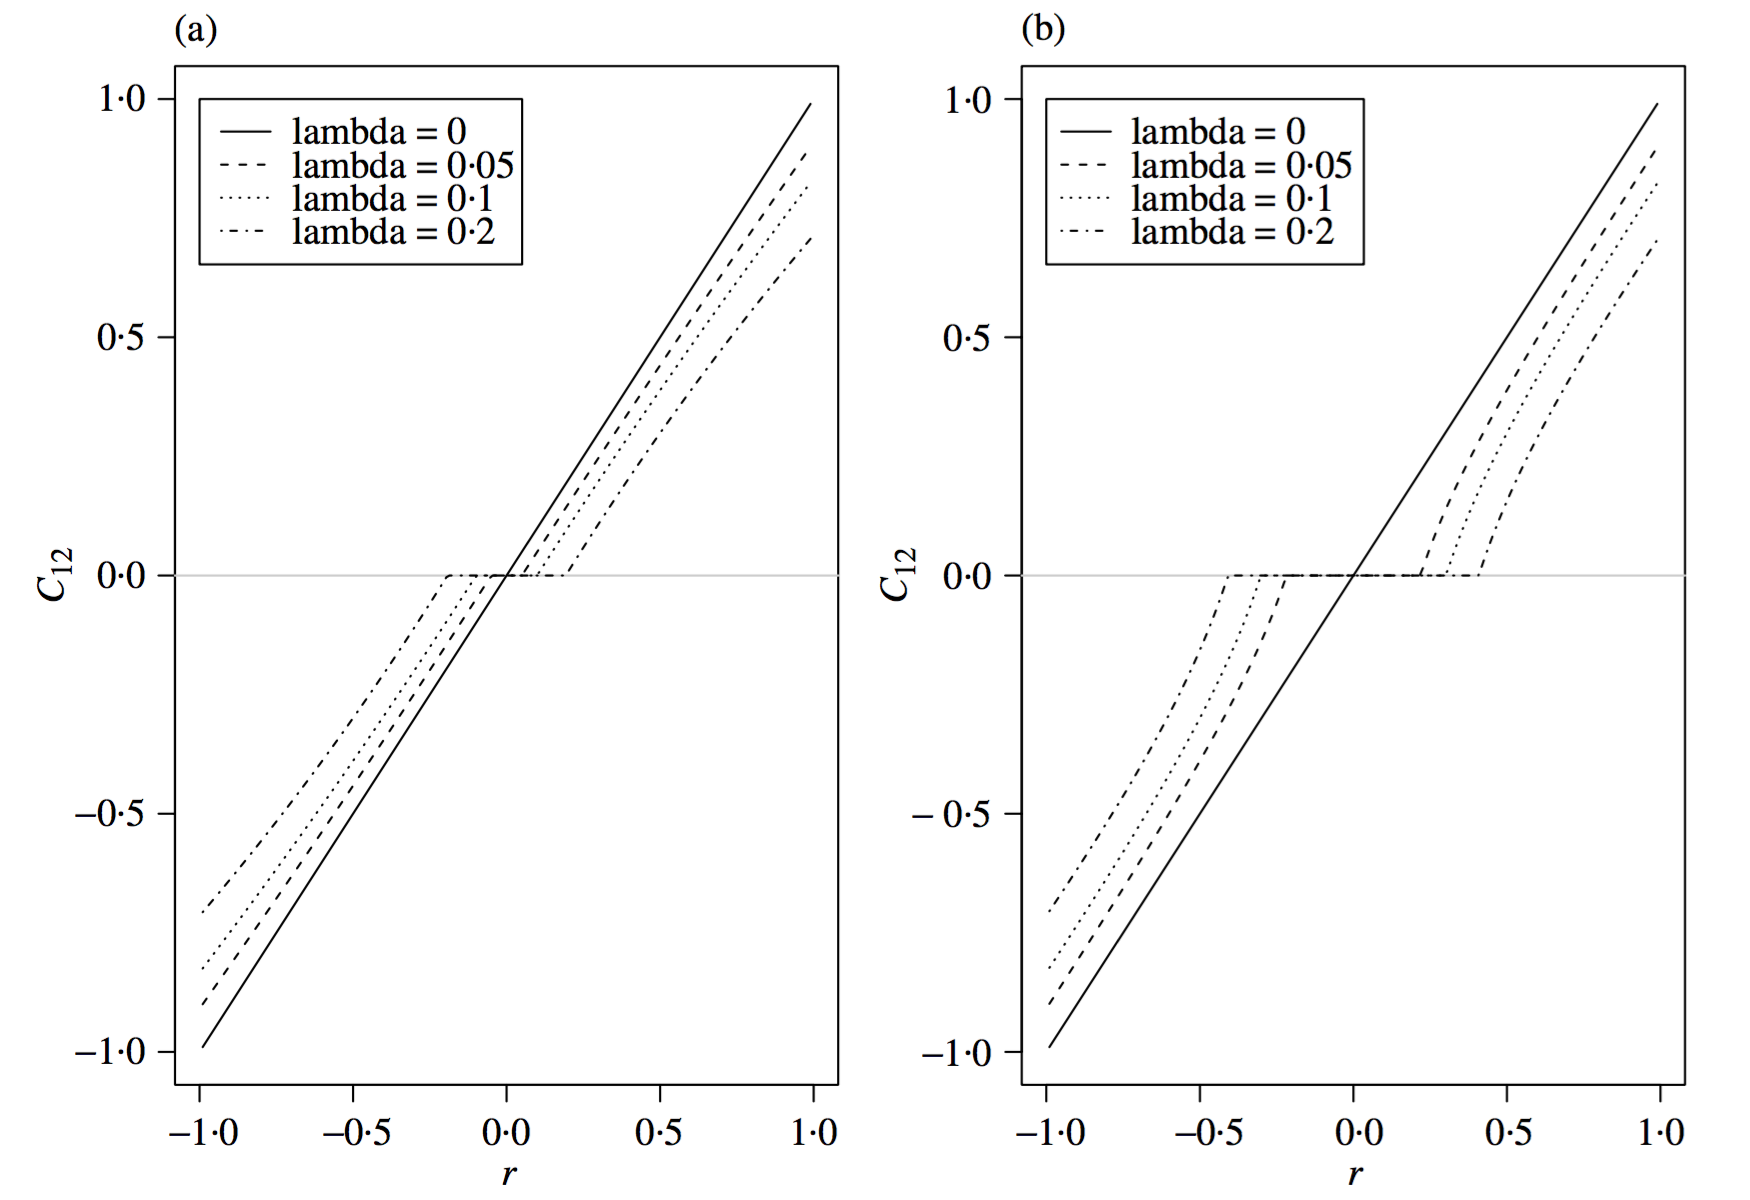
\includegraphics[width=0.75\linewidth]{Fig1}
\captionof{figure}{\color{Green} (a) Lasso-type estimator, (b) garrote-type estimator}
\end{center}